\documentclass[reprint,amsmath,amssymb,aps,]{revtex4-2}
\usepackage{graphicx}
\usepackage{dcolumn}
\usepackage{bm}
\usepackage{scrextend}
\usepackage{vmargin}
\usepackage{multirow}
\usepackage[utf8]{inputenc}
\usepackage[spanish, es-tabla]{babel}
\usepackage{enumerate}
\usepackage{float}
\usepackage{lipsum}
\usepackage{amsmath, amsthm, amssymb, amsfonts}
\usepackage[usenames]{color}
\usepackage[breaklinks=true,hidelinks]{hyperref}
\pagestyle{empty}
\spanishdecimal{.}
\begin{document}
\preprint{APS/123-QED}
\begin{abstract}
\lipsum[1]
\end{abstract}
\begin{titlepage}
\begin{center}

\includegraphics[scale=0.40]{../../../Logos/uanl.png} 
\hspace{2.5cm}

\includegraphics[scale=0.40]{../../../Logos/fcfm.png}
\end{center}
\vspace{2cm}
\begin{center}
\textbf{
UNIVERSIDAD AUTÓNOMA DE NUEVO LEÓN\\
FACULTAD DE CIENCIAS
FÍSICO MATEMÁTICAS}\\
\vspace*{2cm}
\begin{large}
\vspace{1cm}
\large{\textbf{Aplicaciones de la Mecánica Cuántica}}\vspace{1.5cm}\\
\textbf{Tarea 2:\\ Indexación de un patrón de \\difracción de electrones}\\
Carlos Luna\\
\end{large}
\vspace{3.5cm}
\begin{minipage}{0.6\linewidth}
\vspace{0.5cm}
\changefontsizes{14pt}
Nombre:\\
Giovanni Gamaliel López Padilla\\
\end{minipage}
\begin{minipage}{0.2\linewidth}
\changefontsizes{14pt}
Matricula:\\
1837522\\
\end{minipage}
\end{center}
\vspace{4cm}
\begin{flushright}
\today
\end{flushright}
\pagebreak
\end{titlepage}
\maketitle
\section{Introducción}
\lipsum[1]
\section{Objetivo}
Realizar una indexación a un sistema de átomos de plata dado sus parámetros de difracción de electrones.
\section{Marco teórico}
\begin{table}[H]
    \centering
    \begin{tabular}{ccccc}\hline
        2$\theta$ & Intensity & D-Spacing (\r{A}) & HKL & Multiplicity\\ \hline
        38.15 & 100 & 2.3592 & 111 & 8 \\
        44.34 & 46.77 & 2.0431 & 200 & 6 \\
        66.50 & 25.61 & 1.447 & 220 & 12 \\
        77.47 & 27.18 & 1.2320 & 311 & 24 \\
        81.62 & 7.69 & 1.1796 & 222 & 8 \\ \hline
    \end{tabular}
    \caption{Parámetros para el sistema de plata con densidad $\rho=10.500 g/cm^{3}$, irradiado con un haz de $1.541838$\r{A}}
    \label{tabla:parametros}
\end{table}
\begin{figure}[H]
    \centering
    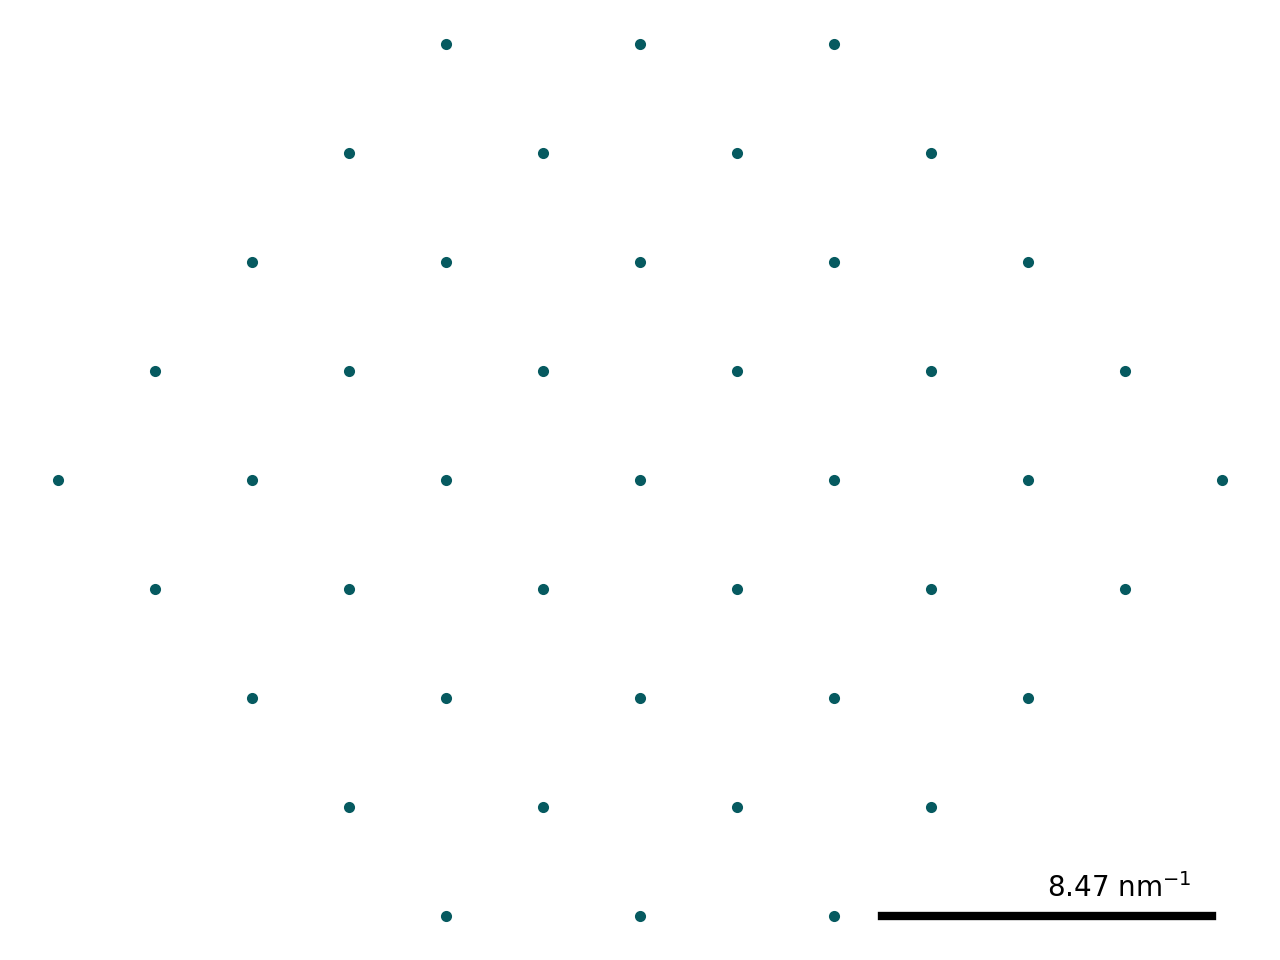
\includegraphics[scale=0.4]{../Graphics/inicial.png}
    \caption{Configuración de los átomos de Plata}
    \label{fig:inicial}
\end{figure}
\section{Resultados}
\begin{figure}[H]
    \centering
    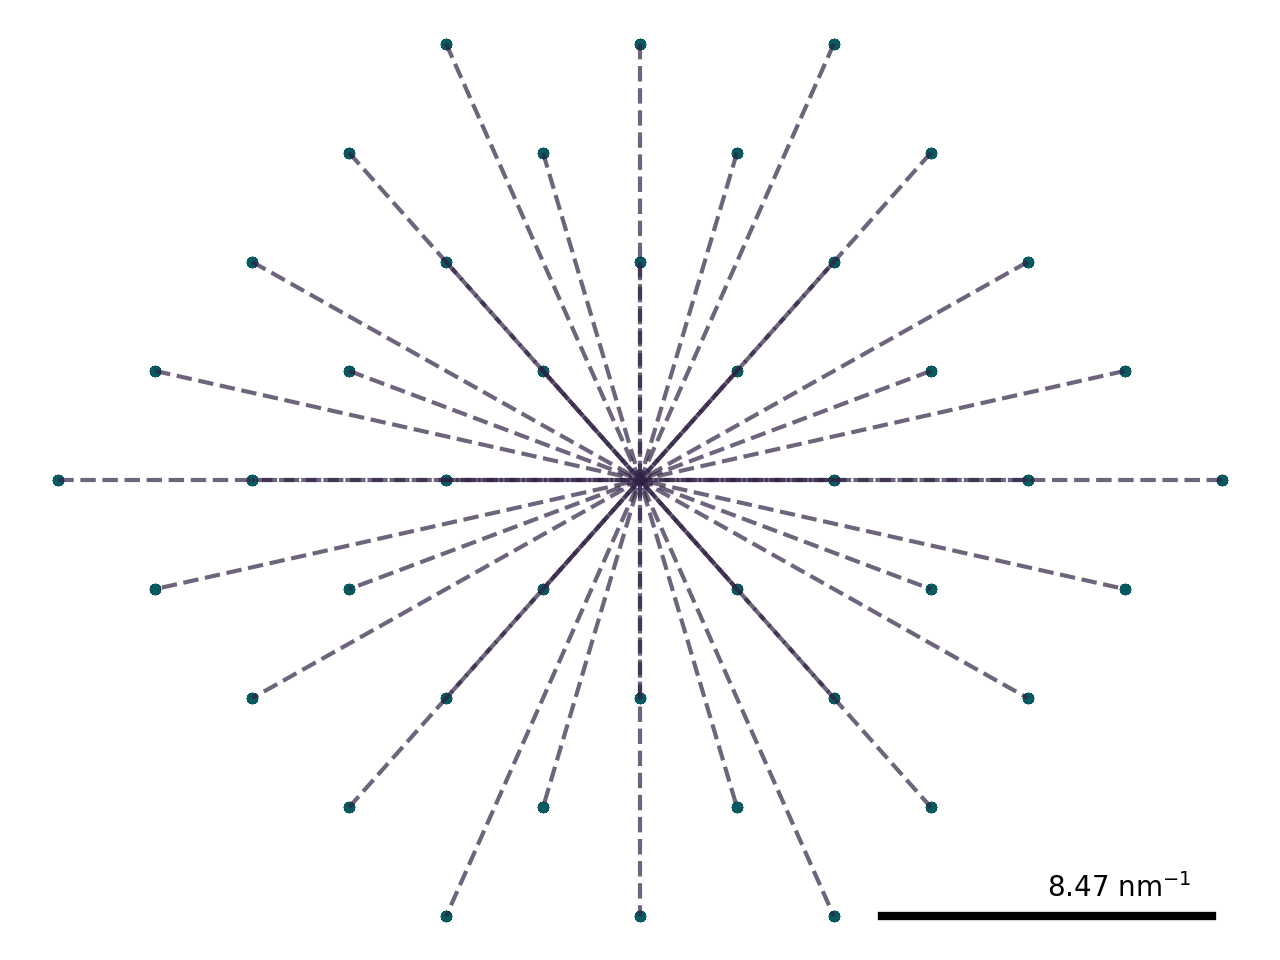
\includegraphics[scale=0.4]{../Graphics/distancia.png}
    \caption{Distancias interatomicas calculadas usando el criterio}
    \label{fig:distancias}
\end{figure}
\begin{figure}[H]
    \centering
    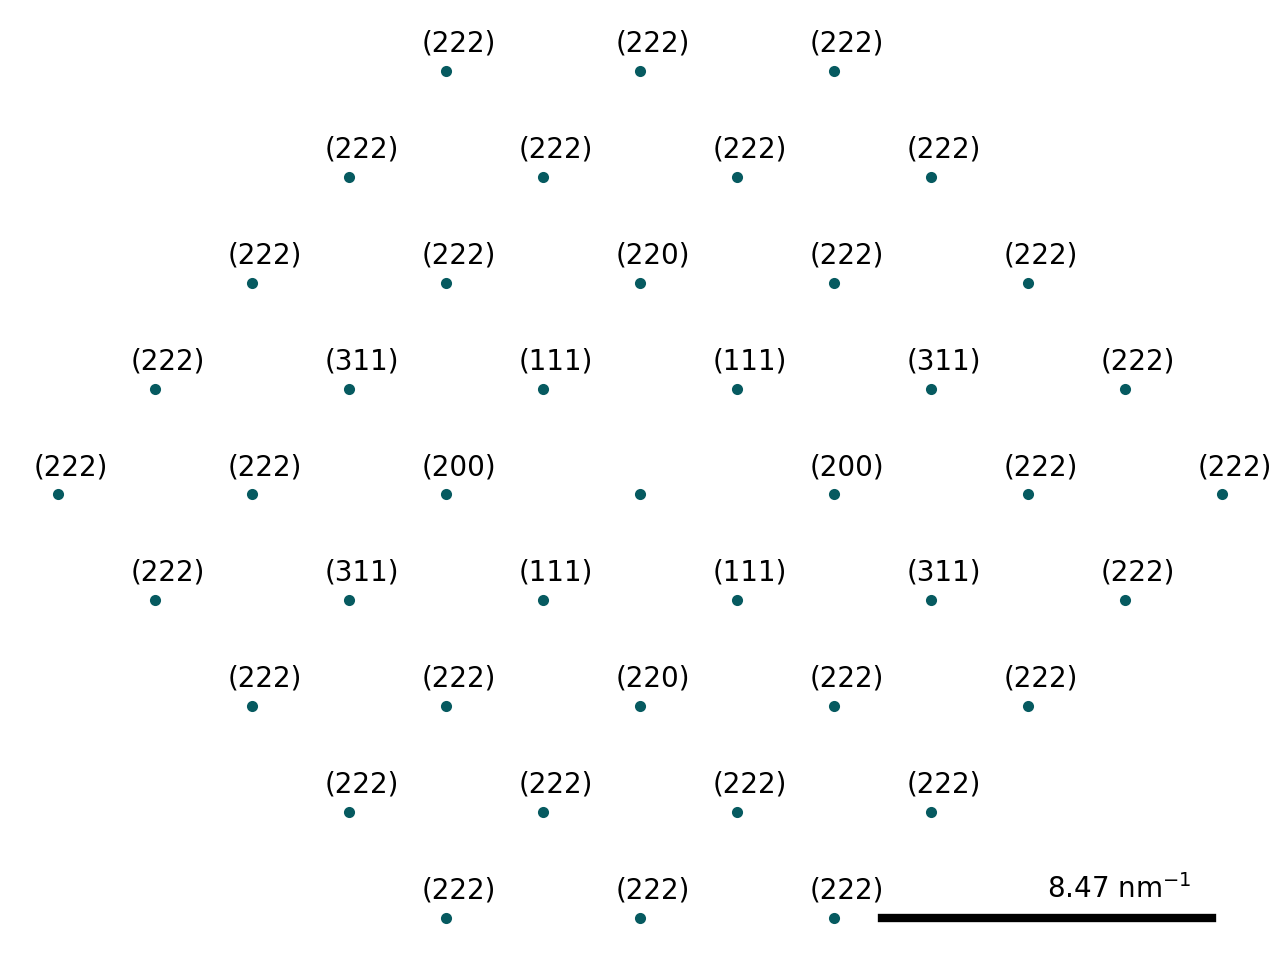
\includegraphics[scale=0.4]{../Graphics/indices.png}
    \caption{Indices de Miller asignados a partir de los datos de la tabla \ref{tabla:parametros} usando el código \ref{cod:distancias}}
    \label{fig:indicesmiller}
\end{figure}
\section{Conclusiones}
\section{Código}
\begin{enumerate}
    \item \href{https://github.com/giovannilopez9808/Notas_Agosto_2020/blob/master/AMC/Tarea2/distancia.py}{Distancia.py\label{cod:distancias}}\\
    Este código realiza las figuras \ref{fig:inicial}, \ref{fig:distancias} y \ref{fig:indicesmiller} a partir de la posición de los átomos y la información de la tabla \ref{tabla:parametros}
\end{enumerate}
\bibliographystyle{plain}
\nocite{*}
\bibliography{Main}
\end{document}